\documentclass[12pt, a4paper]{article}

\usepackage[T1]{fontenc}
\usepackage[utf8]{inputenc}
\usepackage[charter, cal=cmcal]{mathdesign}
\usepackage[scaled=0.92]{helvet}
\usepackage{geometry}
\geometry{a4paper, top=30mm, bottom=30mm, inner=30mm, outer=30mm}

\usepackage{amsmath, amsthm}
\usepackage{amssymb}
\usepackage{xcolor}
\usepackage{tikz}
\usetikzlibrary{arrows.meta, calc}
\usepackage{fancyhdr}
\usepackage{titlesec}
\usepackage{enumitem}
\usepackage{booktabs}
\usepackage{array}
\usepackage{parskip}
\usepackage[colorlinks=true, linkcolor=NavyBlue, urlcolor=NavyBlue, citecolor=NavyBlue]{hyperref}

% ── Colours (Journey 6 — navy blue / gold) ────────────────────────────────────
\definecolor{NavyBlue}{HTML}{1E3A8A}
\definecolor{ModuleColor}{HTML}{2563EB}
\definecolor{PuzzleColor}{HTML}{D97706}
\definecolor{DiscoveryColor}{HTML}{B45309}
\definecolor{ProblemColor}{HTML}{6B21A8}
\definecolor{ReflectColor}{HTML}{0D9488}
\definecolor{LightBlue}{HTML}{EFF6FF}
\definecolor{LightGold}{HTML}{FEF3C7}
\definecolor{LightGreen}{HTML}{ECFDF5}

% ── Custom Environments (No TColorBox for Math style) ─────────────────────────
\newenvironment{puzzlebox}
  {\par\medskip\fillcolorbox{LightGold}{PuzzleColor}{The Puzzle}}
  {\par\medskip}

\newenvironment{discoverybox}
  {\par\medskip\fillcolorbox{LightGreen}{DiscoveryColor}{Discovery}}
  {\par\medskip}

\newenvironment{namedconcept}[1]
  {\par\medskip\fillcolorbox{LightBlue}{NavyBlue}{#1}}
  {\par\medskip}

\newenvironment{reflectionbox}
  {\par\medskip\fillcolorbox{LightBlue}{ReflectColor}{Reflection}}
  {\par\medskip}

\newcommand{\fillcolorbox}[3]{%
  \noindent
  \filldrawbox{#1}{#2}{\textbf{\sffamily\color{white}#3}}\par\nobreak\vspace{4pt}
}

\newcommand{\filldrawbox}[3]{%
  \colorbox{#1}{\parbox{\dimexpr\linewidth-2\fboxsep\relax}{%
    \vspace{4pt}\noindent\hspace{4pt}#3\vspace{4pt}%
  }}%
}

% ── Section formatting ────────────────────────────────────────────────────────
\titleformat{\section}
  {\normalfont\sffamily\Large\bfseries\color{NavyBlue}}
  {\thesection}{1em}{}[\color{NavyBlue!40}{\titlerule[1.5pt]}]
\titleformat{\subsection}
  {\normalfont\sffamily\large\bfseries\color{ModuleColor}}{\thesubsection}{1em}{}

\pagestyle{fancy}
\fancyhf{}
\fancyhead[L]{\small\sffamily\color{NavyBlue}\textit{Discovery Curriculum}}
\fancyhead[R]{\small\sffamily\color{ModuleColor}\textit{Journey 6 $\cdot$ Module 4}}
\fancyfoot[C]{\small\color{NavyBlue}\thepage}
\renewcommand{\headrulewidth}{0.4pt}

\newcommand{\newterm}[1]{\textit{\textcolor{DiscoveryColor}{#1}}}

\begin{document}

\thispagestyle{empty}
\begin{center}
{\small\color{ModuleColor}\textbf{DISCOVERY CURRICULUM}\quad$\cdot$\quad\textbf{JOURNEY 6: ABSTRACTION}}
\vspace{0.6cm}

{\color{NavyBlue}\rule{\linewidth}{2.5pt}}\vspace{0.5cm}

{\Huge\bfseries\color{NavyBlue}Module 4}\\[0.3cm]
{\LARGE\bfseries\color{ModuleColor}Monads and Universal Properties}\\[0.4cm]
{\color{PuzzleColor}\rule{0.4\linewidth}{1.5pt}}\\[0.4cm]
{\large\itshape\color{NavyBlue!80}
Objects can be characterized by their elements or their relationships.\\[0.15cm]
Universal properties define structures up to unique isomorphism.\\[0.15cm]
Monads formalize the wrapping and flattening of computational context.}

\vspace{1.4cm}
\begin{tabular}{rl}
\textbf{Journey}         & Journey 6 --- Abstraction \\[4pt]
\textbf{Module}          & 4 of 4 \\[4pt]
\textbf{Prerequisites}   & Module 6.3 (categories, functors, natural transformations) \\[4pt]
\textbf{You will discover} & Universal properties, limits, colimits, monads, adjunctions \\[4pt]
\textbf{Format}          & 8 problems $+$ 2 deep problems $\approx$ 13 pages \\
\end{tabular}
\vspace{1.2cm}

{\color{NavyBlue}\rule{\linewidth}{2.5pt}}
\end{center}

\newpage

\section{Module 6.4 --- Monads and Universal Properties}
\label{sec:mod6.4}

\subsection*{Motivation}

We formalized in Module 6.3 the basic grammar of Category Theory: objects, morphisms, functors, and natural transformations.
Now, we complete this journey of abstraction by studying how we define mathematical constructions not by their internal elements, but entirely by their external relationships.
These definitions are **Universal Properties**.

Universal properties allow us to define Cartesian products, quotients, and intersections across any category using commuting diagrams.
Finally, we explore **Monads**, a concept first introduced by Roger Godement in 1958.
A monad is an algebraic structure on a functor that formalizes the process of wrapping values in a context and flattening nested contexts.
In doing so, monads bridge the boundary between pure mathematics and computer science, providing the formal semantic foundation for handling side-effects, state, and nullability in modern programming.

\subsection{Characterizing by Arrows}

We analyze why defining objects by their incoming and outgoing morphisms is superior to element-based definitions.

\begin{puzzlebox}
In set theory, we define the Cartesian product of two sets $A$ and $B$ as the set of ordered pairs:
\[
  A \times B \;=\; \{(a, b) : a \in A, b \in B\}.
\]
However, we can characterize this product without ever mentioning its elements.
* Let $A \times B$ be an object equipped with two projection maps $p_A: A \times B \to A$ and $p_B: A \times B \to B$.
* We state: For *any* other object $C$ equipped with maps $f: C \to A$ and $g: C \to B$, there exists a *unique* morphism $h: C \to A \times B$ such that $p_A \circ h = f$ and $p_B \circ h = g$.
\begin{center}
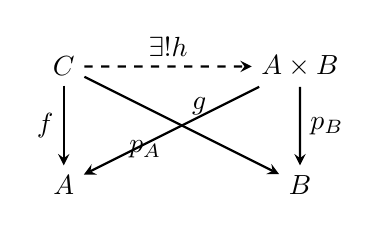
\begin{tikzpicture}[scale=1.5]
  \node (C) at (0,1) {$C$};
  \node (P) at (2,1) {$A \times B$};
  \node (A) at (0,0) {$A$};
  \node (B) at (2,0) {$B$};
  
  \draw[->, >=stealth, dashed, thick] (C) -- node[above] {$\exists! h$} (P);
  \draw[->, >=stealth, thick] (C) -- node[left] {$f$} (A);
  \draw[->, >=stealth, thick] (P) -- node[right] {$p_B$} (B);
  \draw[->, >=stealth, thick] (P) -- node[below left] {$p_A$} (A);
  \draw[->, >=stealth, thick] (C) -- node[above right] {$g$} (B);
\end{tikzpicture}
\end{center}
\begin{enumerate}[label=(\alph*), leftmargin=*]
  \item Show that if $C = A \times B$, the unique morphism $h$ is the identity morphism.
  \item Why does this arrow-based definition (a **universal property**) define the product uniquely up to a unique isomorphism?
  \item In the category of Groups ($\mathbf{Grp}$), what group construction satisfies this exact same universal property? (What is the "product" group?)
\end{enumerate}
\end{puzzlebox}

\subsection{Limits and Colimits}

We generalize products, intersections, and quotients into universal shapes.

\begin{namedconcept}{Limits and Colimits}
A universal property defines either a limit (generalizing products and intersections) or a colimit (generalizing unions and quotients).
* **The Coproduct (Colimit):** The coproduct of $A$ and $B$ is an object $A + B$ with injections $i_A: A \to A+B$ and $i_B: B \to A+B$ such that for any object $C$ with maps $f: A \to C$ and $g: B \to C$, there is a unique $h: A+B \to C$ making the diagram commute.
\begin{center}
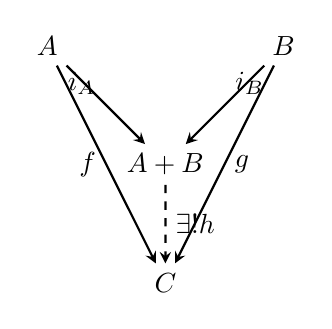
\begin{tikzpicture}[scale=1.5]
  \node (A) at (0,1) {$A$};
  \node (B) at (2,1) {$B$};
  \node (P) at (1,0) {$A + B$};
  \node (C) at (1,-1) {$C$};
  
  \draw[->, >=stealth, thick] (A) -- node[above left] {$i_A$} (P);
  \draw[->, >=stealth, thick] (B) -- node[above right] {$i_B$} (P);
  \draw[->, >=stealth, thick] (A) -- node[left] {$f$} (C);
  \draw[->, >=stealth, thick] (B) -- node[right] {$g$} (C);
  \draw[->, >=stealth, dashed, thick] (P) -- node[right] {$\exists! h$} (C);
\end{tikzpicture}
\end{center}
\end{namedconcept}

\begin{enumerate}[label=(\alph*), leftmargin=*]
  \item In the category $\mathbf{Set}$, show that the coproduct $A + B$ is the **disjoint union** of the two sets.
  \item In the category of Abelian Groups ($\mathbf{Ab}$), what group construction satisfies the coproduct universal property? (Is it the direct sum?)
\end{enumerate}

\subsection{Monads: Functors with Algebra}

We formalize the wrapping and flattening of structure.

\begin{namedconcept}{Monads}
A \newterm{monad} on a category $\mathcal{C}$ is an endofunctor $T: \mathcal{C} \to \mathcal{C}$ equipped with two natural transformations:
1. **Unit ($\eta: \text{Id}_{\mathcal{C}} \Rightarrow T$):** A mapping that wraps a raw value into the monad's context.
2. **Multiplication ($\mu: T^2 \Rightarrow T$):** A mapping that flattens a nested context $T(T(X))$ into a single context $T(X)$.

These must satisfy the following coherence equations (associativity and unit laws):
\[
  \mu \circ T\mu \;=\; \mu \circ \mu_T, \qquad \mu \circ T\eta \;=\; \mu \circ \eta_T \;=\; \text{id}_T.
\]
\end{namedconcept}

\begin{enumerate}[label=(\alph*), leftmargin=*]
  \item Let the functor $T$ be the **List functor** on $\mathbf{Set}$, mapping a set $X$ to the set of all lists of elements in $X$.
        Identify the unit $\eta_X(x)$ and the multiplication $\mu_X(\text{list of lists})$.
  \item Explain why $\mu_X$ represents the standard list "flatten" (concatenation) operation.
  \item Write down the associativity law for the List monad using a list of lists of lists: $L(L(L(X)))$.
\end{enumerate}

\subsection{The Monad Bridge to Computing}

We study how category-theoretic monads model side-effects in programming.

\begin{explobox}
In pure functional programming, functions must be mathematically pure: they take an input and return an output with zero side-effects (no state changes, no exceptions, no I/O).
\problem We use monads to model side-effects cleanly:
* **The Maybe Monad:** Models computations that can fail (nullability). The functor is $T(X) = X \cup \{\text{Nothing}\}$. The unit wraps a value: $\eta(x) = \text{Just}(x)$.
* **The State Monad:** Models mutable state. The functor is $T(X) = S \to (X \times S)$, mapping a state input to a value and a new state.
\begin{enumerate}[label=(\alph*), leftmargin=*]
  \item Suppose we have nested nullable operations: getting a user profile, then their address, then their zip code. Each step can return `Nothing`.
        Without a monad, we must write nested `if-else` blocks to check for null.
        Explain how the multiplication (flattening) operation of the Maybe monad allows us to chain these operations cleanly, bypassing the nested checks.
  \item In computer science, the bind operation is defined as $x \gg= f = \mu(T(f)(x))$.
        Show that this bind operation is a direct consequence of the monad axioms.
\end{enumerate}
\end{explobox}

\newpage

\section{Part 3 --- Discovery}

\begin{discoverybox}
\textbf{What have we built?}

\textbf{First.} A universal property characterizes a mathematical object uniquely up to a unique isomorphism by its incoming or outgoing morphisms.

\textbf{Second.} Cartesian products and intersections are limits. Disjoint unions and quotients are colimits.

\textbf{Third.} A monad is an endofunctor equipped with natural transformations for unit ($\eta$) and multiplication ($\mu$) that govern the wrapping and flattening of structural context.

\textbf{Fourth.} Monads bridge mathematics and computing, formalizing side-effects (state, I/O, exceptions) within pure functional programming languages.
\end{discoverybox}

\newpage

\section{Part 4 --- What This Is Called}

\begin{namedconcept}{Category Monad Parameters}
* **Universal Property:** A property characterizing an object as the unique terminal or initial object in a auxiliary category of maps.
* **Limit:** The universal object representing the dome of a diagram of morphisms (generalizing products).
* **Colimit:** The dual universal object representing the basin of a diagram (generalizing coproducts).
* **Monad:** An algebraic triple $(T, \eta, \mu)$ on an endofunctor satisfying associativity and unit coherence laws.
* **Adjunction:** A pair of adjoint functors $F \dashv G$ that represent a weak equivalence of categories.
\end{namedconcept}

\newpage

\section{Part 5 --- Solved Exercises}

\begin{enumerate}[label=\textbf{E\arabic*.}]
  \item \textbf{Uniqueness of Products up to Isomorphism.}
  
        Prove that if $P$ and $Q$ are both products of two objects $A$ and $B$ in a category $\mathcal{C}$, then $P \cong Q$ via a unique isomorphism that commutes with the projections.
        
        \textbf{Solution:}
        Let $P$ be a product of $A$ and $B$, equipped with projection maps $p_A: P \to A$ and $p_B: P \to B$.
        Let $Q$ be a product of $A$ and $B$, equipped with projection maps $q_A: Q \to A$ and $q_B: Q \to B$.
        
        1. **Constructing the maps:**
           Since $P$ is a product, and $Q$ is equipped with maps $q_A: Q \to A$ and $q_B: Q \to B$, the universal property of $P$ states that there exists a unique morphism $h_1: Q \to P$ such that:
           \[
             p_A \circ h_1 \;=\; q_A, \qquad \text{and} \qquad p_B \circ h_1 \;=\; q_B.
           \]
           Similarly, since $Q$ is a product and $P$ is equipped with maps $p_A: P \to A$ and $p_B: P \to B$, the universal property of $Q$ states that there exists a unique morphism $h_2: P \to Q$ such that:
           \[
             q_A \circ h_2 \;=\; p_A, \qquad \text{and} \qquad q_B \circ h_2 \;=\; p_B.
           \]
        
        2. **Composing the maps:**
           Now, evaluate the composition $h_1 \circ h_2: P \to P$.
           Using the relations:
           \[
             p_A \circ (h_1 \circ h_2) \;=\; (p_A \circ h_1) \circ h_2 \;=\; q_A \circ h_2 \;=\; p_A.
           \]
           \[
             p_B \circ (h_1 \circ h_2) \;=\; (p_B \circ h_1) \circ h_2 \;=\; q_B \circ h_2 \;=\; p_B.
           \]
           Thus, the map $h_1 \circ h_2$ commutes with the projections of $P$.
           However, by the universal property of $P$ using the maps $p_A$ and $p_B$, there exists a *unique* map $h: P \to P$ satisfying $p_A \circ h = p_A$ and $p_B \circ h = p_B$.
           The identity map $\text{id}_P$ clearly satisfies this condition.
           Therefore, by uniqueness:
           \[
             h_1 \circ h_2 \;=\; \text{id}_P.
           \]
           By a symmetric argument, evaluating the composition $h_2 \circ h_1: Q \to Q$, we find:
           \[
             h_2 \circ h_1 \;=\; \text{id}_Q.
           \]
           
        Since $h_1 \circ h_2 = \text{id}_P$ and $h_2 \circ h_1 = \text{id}_Q$, the morphism $h_1$ is an isomorphism with inverse $h_2$.
        Thus, $P \cong Q$ via a unique isomorphism.
        
  \item \textbf{Coherence Diagrams of a Monad.}
  
        Write down the commuting diagrams that represent the associativity and unit axioms of a monad $(T, \eta, \mu)$.
        
        \textbf{Solution:}
        1. **Associativity Law:**
           This law states that flattening a nested context of three layers $T^3(X)$ can be done in two ways, both yielding the same result. The following diagram must commute:
           \begin{center}
           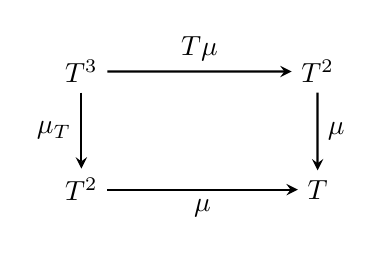
\begin{tikzpicture}[scale=1.5]
             \node (T3) at (0,1) {$T^3$};
             \node (T2_1) at (2,1) {$T^2$};
             \node (T2_2) at (0,0) {$T^2$};
             \node (T) at (2,0) {$T$};
             
             \draw[->, >=stealth, thick] (T3) -- node[above] {$T\mu$} (T2_1);
             \draw[->, >=stealth, thick] (T3) -- node[left] {$\mu_T$} (T2_2);
             \draw[->, >=stealth, thick] (T2_1) -- node[right] {$\mu$} (T);
             \draw[->, >=stealth, thick] (T2_2) -- node[below] {$\mu$} (T);
           \end{tikzpicture}
           \end{center}
           Equation: $\mu \circ T\mu = \mu \circ \mu_T$.
           
        2. **Unit Laws:**
           These laws state that wrapping a value inside the monad's context and then flattening it returns the original value. The following diagram must commute:
           \begin{center}
           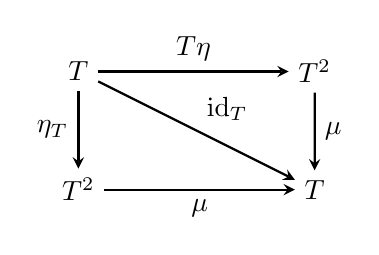
\begin{tikzpicture}[scale=1.5]
             \node (T) at (0,1) {$T$};
             \node (T2_1) at (2,1) {$T^2$};
             \node (T2_2) at (0,0) {$T^2$};
             \node (T_out) at (2,0) {$T$};
             
             \draw[->, >=stealth, thick] (T) -- node[above] {$T\eta$} (T2_1);
             \draw[->, >=stealth, thick] (T) -- node[left] {$\eta_T$} (T2_2);
             \draw[->, >=stealth, thick] (T2_1) -- node[right] {$\mu$} (T_out);
             \draw[->, >=stealth, thick] (T2_2) -- node[below] {$\mu$} (T_out);
             \draw[->, >=stealth, thick] (T) -- node[above right] {$\text{id}_T$} (T_out);
           \end{tikzpicture}
           \end{center}
           Equation: $\mu \circ T\eta = \mu \circ \eta_T = \text{id}_T$.
\end{enumerate}

\newpage

\section{Part 6 --- Problems}

\begin{enumerate}[label=\textbf{P\arabic*.}]
  \item \textbf{The Coproduct Universal Property.}
  
        The coproduct of $A$ and $B$ is the dual construction of the product, reversing all arrows.
        \begin{enumerate}[label=(\alph*)]
          \item Write down the universal property of the coproduct in your own words. Draw the commuting diagram.
          \item In the category $\mathbf{Set}$, the coproduct is the disjoint union:
          \[
            A + B \;=\; (A \times \{0\}) \cup (B \times \{1\}).
          \]
          Define the injection maps $i_A: A \to A+B$ and $i_B: B \to A+B$ for this set construction.
          \item Show that for any set $C$ and functions $f: A \to C$ and $g: B \to C$, the unique function $h: A+B \to C$ is:
          \[
            h(x, 0) \;=\; f(x), \qquad h(y, 1) \;=\; g(y).
          \]
        \end{enumerate}

  \item \textbf{The List Monad.}
  
        The List construction defines a monad $(L, \eta, \mu)$ on the category $\mathbf{Set}$.
        \begin{enumerate}[label=(\alph*)]
          \item For a set $X$, the unit $\eta_X: X \to L(X)$ maps an element $x \in X$ to a list. Define this mapping.
          \item The multiplication $\mu_X: L(L(X)) \to L(X)$ takes a list of lists and flattens it.
                If $S = [[1, 2], [], [3, 4]] \in L(L(\mathbb{Z}))$, calculate $\mu_{\mathbb{Z}}(S)$.
          \item The list functor maps a function $f: X \to Y$ to $L(f): L(X) \to L(Y)$ by applying $f$ to every element in the list (the `map` function).
                Show that the naturality condition $\mu_Y \circ L(L(f)) = L(f) \circ \mu_X$ holds.
        \end{enumerate}
\end{enumerate}

\newpage

\section{Part 7 --- Deep Problems}

\begin{enumerate}[label=\textbf{D\arabic*.}]
  \item \textbf{Monads from Adjunctions.}
  
        A pair of adjoint functors $F: \mathcal{C} \to \mathcal{D}$ (left adjoint) and $G: \mathcal{D} \to \mathcal{C}$ (right adjoint), written $F \dashv G$, is defined by a natural bijection:
        \[
          \phi_{X,Y}: \text{Hom}_{\mathcal{D}}(F(X), Y) \;\cong\; \text{Hom}_{\mathcal{C}}(X, G(Y)).
        \]
        This bijection yields a unit natural transformation $\eta: \text{Id}_{\mathcal{C}} \Rightarrow G \circ F$ and a counit $\varepsilon: F \circ G \Rightarrow \text{Id}_{\mathcal{D}}$.
        \begin{enumerate}[label=(\alph*)]
          \item Let $T = G \circ F$ be the composed endofunctor on $\mathcal{C}$.
                Prove that $T$ is a functor.
          \item We define the multiplication natural transformation $\mu: T^2 \Rightarrow T$ by:
                \[
                  \mu_X \;=\; G(\varepsilon_{F(X)}): G(F(G(F(X)))) \to G(F(X)).
                \]
                Explain why $G(\varepsilon_{F(X)})$ has the correct domain and codomain to act as the multiplication of the monad.
          \item Using the triangle identities for adjunctions:
                \[
                  \varepsilon_F \circ F\eta \;=\; \text{id}_F \qquad \text{and} \qquad G\varepsilon \circ \eta_G \;=\; \text{id}_G,
                \]
                prove the monad unit coherence law: $\mu \circ T\eta = \text{id}_T$.
        \end{enumerate}

  \item \textbf{Equalizers as Limits.}
  
        Let $f, g: A \to B$ be two parallel morphisms in a category $\mathcal{C}$.
        An **equalizer** of $f$ and $g$ is an object $E$ together with a morphism $\text{eq}: E \to A$ such that $f \circ \text{eq} = g \circ \text{eq}$.
        \begin{enumerate}[label=(\alph*)]
          \item State the universal property of the equalizer: for any object $Z$ with a map $h: Z \to A$ satisfying $f \circ h = g \circ h$, there exists a unique map $k: Z \to E$ making the diagram commute. Draw this commuting diagram.
          \item In the category $\mathbf{Set}$, prove that the equalizer is isomorphic to the subset:
          \[
            E \;=\; \{x \in A : f(x) = g(x)\}.
          \]
          Specify the map $\text{eq}$ in this set construction.
          \item In the category of Vector Spaces ($\mathbf{Vect}_K$), let $g: A \to B$ be the zero map ($g(x) = 0$).
                Show that the equalizer of a linear map $f: A \to B$ and the zero map $g$ is isomorphic to the **kernel** of $f$.
                Why does this show that kernels are a special case of category-theoretic limits?
        \end{enumerate}
\end{enumerate}

\newpage

\section{Part 8 --- Reflection}

\begin{reflectionbox}
\textbf{Conceptual Reflection}

Consider the following questions:
\begin{enumerate}
  \item **On the Arrow Philosophy:** Universal properties define objects solely by their relations (arrows) rather than their internal contents. If we can define all mathematical objects by their relations, does this mean that "substance" is an illusion, and only "relationship" is real?
  \item **On Adjunctions:** Mac Lane stated that "adjoint functors arise everywhere." An adjunction represents a weak equivalence—a way of translating a problem between two different categories (like Sets and Groups) without losing structural information. Why is translating problems between different domains such a powerful problem-solving method?
  \item **On Computing and Algebra:** We saw that monads in computer science are exactly the monads of category theory. Why does pure, abstract mathematics (which had no conception of computers in 1945) serve as the absolute, perfect guide for designing safe, modern programming languages?
\end{enumerate}
\end{reflectionbox}

\medskip
\noindent\textbf{Looking ahead.}
Module~6.5 introduces **Group Representation Theory**. Having mastered category theory and abstract group relationships, we will explore how groups act on vector spaces to linearize symmetry, bridging abstract algebra directly to quantum mechanics and physical symmetries.

\vspace{1.4cm}
\begin{center}
{\color{NavyBlue}\rule{0.5\linewidth}{0.8pt}}\\[6pt]
{\small\color{NavyBlue}\textit{End of Journey 6, Module 6.4 --- Monads and Universal Properties}}\\[4pt]
{\small\color{NavyBlue}Continue to: \textbf{Module 6.5 --- Group Representation Theory}}\\[6pt]
{\color{NavyBlue}\rule{0.5\linewidth}{0.8pt}}
\end{center}

\end{document}
